%%%%%%%%%%%%%%%%%%%%%%%%%%%%%%%%%%%%%%%%%
% Beamer Presentation
% LaTeX Template
% Version 1.0 (10/11/12)
%
% This template has been downloaded from:
% http://www.LaTeXTemplates.com
%
% License:
% CC BY-NC-SA 3.0 (http://creativecommons.org/licenses/by-nc-sa/3.0/)
%
%%%%%%%%%%%%%%%%%%%%%%%%%%%%%%%%%%%%%%%%%

% ----------------------------------------------------------------------------------------
% PACKAGES AND THEMES
% ----------------------------------------------------------------------------------------

\documentclass{beamer}

\mode<presentation> {

  % The Beamer class comes with a number of default slide themes
  % which change the colors and layouts of slides. Below this is a list
  % of all the themes, uncomment each in turn to see what they look like.

  % \usetheme{default}
  % \usetheme{AnnArbor}
  % \usetheme{Antibes}
  % \usetheme{Bergen}
  % \usetheme{Berkeley}
  % \usetheme{Berlin}
  % \usetheme{Boadilla}
  % \usetheme{CambridgeUS}
  % \usetheme{Copenhagen}
  % \usetheme{Darmstadt}
  % \usetheme{Dresden}
  % \usetheme{Frankfurt}
  % \usetheme{Goettingen}
  % \usetheme{Hannover}
  % \usetheme{Ilmenau}
  % \usetheme{JuanLesPins}
  % \usetheme{Luebeck}
  \usetheme{Madrid}
  % \usetheme{Malmoe}
  % \usetheme{Marburg}
  % \usetheme{Montpellier}
  % \usetheme{PaloAlto}
  % \usetheme{Pittsburgh}
  % \usetheme{Rochester}
  % \usetheme{Singapore}
  % \usetheme{Szeged}
  % \usetheme{Warsaw}

  % As well as themes, the Beamer class has a number of color themes
  % for any slide theme. Uncomment each of these in turn to see how it
  % changes the colors of your current slide theme.

  % \usecolortheme{albatross}
  \usecolortheme{beaver}
  % \usecolortheme{beetle}
  % \usecolortheme{crane}
  % \usecolortheme{dolphin}
  % \usecolortheme{dove}
  % \usecolortheme{fly}
  % \usecolortheme{lily}
  % \usecolortheme{orchid}
  % \usecolortheme{rose}
  % \usecolortheme{seagull}
  % \usecolortheme{seahorse}
  % \usecolortheme{whale}
  % \usecolortheme{wolverine}

  % \setbeamertemplate{footline} % To remove the footer line in all slides uncomment this line
  % \setbeamertemplate{footline}[page number] % To replace the footer line in all slides with a simple slide count uncomment this line

  % \setbeamertemplate{navigation symbols}{} % To remove the navigation symbols from the bottom of all slides uncomment this line
}

\usepackage{graphicx} % Allows including images
\usepackage{booktabs} % Allows the use of \toprule, \midrule and \bottomrule in tables
% draw shit
\usepackage{tikz}
\usetikzlibrary{fit,arrows,calc,positioning}

\graphicspath{{imgs/}}

% ----------------------------------------------------------------------------------------
% TITLE PAGE
% ----------------------------------------------------------------------------------------

\title[Tensorflow Workshop]{Tensorflow Workshop} % The short title appears at the bottom of every slide, the full title is only on the title page

\author{Shotaro Ikeda \& Akshay Mishra} % Your name
\institute[SIGAI] % Your institution as it will appear on the bottom of every slide, may be shorthand to save space
{
  \textit{http://sigai.ml} % Your email address
}
\date{\today} % Date, can be changed to a custom date

\begin{document}

\begin{frame}
  \titlepage % Print the title page as the first slide
\end{frame}

\begin{frame}
  \frametitle{Overview} % Table of contents slide, comment this block out to remove it
  \tableofcontents % Throughout your presentation, if you choose to use \section{} and \subsection{} commands, these will automatically be printed on this slide as an overview of your presentation
\end{frame}

% ----------------------------------------------------------------------------------------
% PRESENTATION SLIDES
% ----------------------------------------------------------------------------------------

% ------------------------------------------------
\section{Basic Tensorflow}

\begin{frame}
  \Huge{\centerline{Basic Tensorflow}}
\end{frame}

\begin{frame}
  \frametitle{Remarks about Tensorflow}
  \begin{itemize}
  \item Quite overwhelming, especially for those new to the library.
  \item There is multiple ways of doing the same thing.
  \item Very different way of thinking vs. other libraries.
  \end{itemize}
\end{frame}

\begin{frame}
  \frametitle{Nice Things about Tensorflow}
  \begin{itemize}
  \item Very fast computation on GPUs (nearly $~80x$ faster than CPU).
  \item Great distributed support for \textbf{large} clusters ($\geq 8$ GPUs).
  \item Many available implementations.
  \end{itemize}
\end{frame}

\subsection{Computational Graphs}

\begin{frame}
  \frametitle{Tensorflow ``Quirks''/Vocabulary}
  \begin{itemize}
  \item \underline{Define and Run}, instead of immediate feedback.
  \item \underline{Placeholders} to transfer data into the computational graph.
  \item \underline{Variables} for values/weights we want to learn.
  \item \underline{Ops} to operate on individual Variables/Values
  \item \underline{Session} to allocate the computational graph, and assign values
  \end{itemize}
\end{frame}

\begin{frame}
  \frametitle{Computational Graphs}
  \begin{itemize}
  \item Let's say we want to compute some values, given variables $x$, $y$, and $z$.
  \item $x \in \mathcal{R}^{2 \times 3}$
  \item $y \in \mathcal{R}^{3 \times 1}$
  \item $z \in \mathcal{R}^{2 \times 1}$
  \item Let's try to compute \textsc{Mean}$(xy + z)$
  \end{itemize}
\end{frame}

%%%%%%%%%%%%%%%%%%%%%%%
% Define and Run Demo %
%%%%%%%%%%%%%%%%%%%%%%%

\begin{frame}
  \frametitle{Demo -- Calculations in Tensorflow}
  \Huge{\centerline{\href{https://github.com/sig-ai/tf_workshop/blob/master/demos/basics.ipynb}{demos/basics.ipynb}}}
\end{frame}

\begin{frame}
  \frametitle{Example -- Conclusions}
  \begin{itemize}
  \item In order to run any computation in Tensorflow, you need a \underline{Session}.
    \begin{itemize}
    \item You need to define the computational graph first
    \item Then initalize your variables and session.
    \end{itemize}
  \item Tensorflow batching is very easy to do, and fast on GPUs
  \end{itemize}
\end{frame}

\section{Review: Supervised Learning}

\begin{frame}
  \Huge{\centerline{Review: Supervised Learning}}
\end{frame}

\subsection{Review: Problem Statement}
\begin{frame}
  \frametitle{Supervised Learning - Problem Statement}
  \begin{itemize}
  \item We have some dataset $d \thicksim \mathcal{D}$.
  \item $d$ contains a bunch of points, $x_i$ and $y_i$, where $x_i$ is the $i$th datapoint and $y_i$ is the $i$th label
  \item You can think of $x_i$ as an image, and $y_i$ being the corresponding label.
  \item Given enough $x_i$'s and $y_i$'s, is it possible to accurately predict $\hat{y}$ for some foreign, unseen inputs $\hat{x}$?
  \end{itemize}
\end{frame}

\begin{frame}
  \frametitle{Supervised Learning - Problem Statement}
  \begin{itemize}
  \item Idea: suppose there exists some function $f$, such that $f: a \rightarrow b$, essentially mapping our inputs $x$ to output $y$.
  \item For the workshop today, this $f$ is approximated by Tensorflow.
  \end{itemize}
\end{frame}

\begin{frame}
  \frametitle{Typical Deep Network Pipeline}
  \tikzstyle{b} = [rectangle, draw, fill=blue!20, node distance=1cm, text width=6em, text centered, rounded corners, minimum height=2em, thick]
  \tikzstyle{n} = [rectangle, draw, fill=purple!20, node distance=1cm, text width=6em, text centered, rounded corners, minimum height=2em, thick]
  \tikzstyle{c} = [rectangle, draw, inner sep=0.5cm, dashed]

  \begin{tikzpicture}[auto]
    \node [b] (input) {Input $x_{i}, y_{i}$};
    % Deep Network
    \node [n, above right = 1cm of input] (deepnet) {Model $f$};

    \node [b, right = 0.5cm of deepnet] (prediction) {Prediction $\hat{y_i}$};
    \node [b, below right = 1cm of prediction] (loss) {Loss};

    \draw [thick,->] (input) -- (deepnet) node [pos=0.5, below] {$x_i$};
    \draw [thick,->] (deepnet) -- (prediction);
    \draw [thick,->] (prediction) -- (loss) node [pos=0.2, below] {$\hat{y_i}$};
    \draw [thick,->] (input) -- (loss) node [pos=0.5, below] {$y_i$};
  \end{tikzpicture}
\end{frame}

\begin{frame}
  \frametitle{Examples of Supervised Learning}
  \begin{figure}
    \includegraphics[width=0.8\linewidth]{mscoco.png}
  \end{figure}
\end{frame}

\begin{frame}
  \frametitle{Examples of Supervised Learning}
  \begin{figure}
    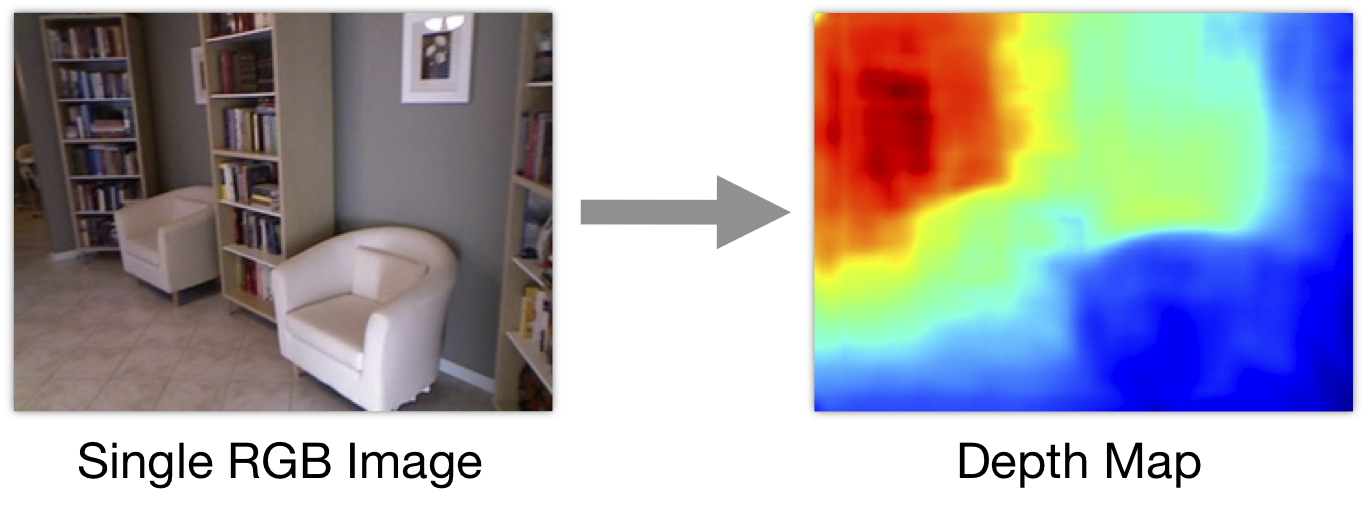
\includegraphics[width=0.8\linewidth]{depth_prediction.png}
  \end{figure}
\end{frame}


% ------------------------------------------------

% ------------------------------------------------
\section{Supervised Learning in Tensorflow}
\subsection{Linear Regression/Classification}


\begin{frame}
  \frametitle{Linear Regression/Classification}
  \begin{block}{Linear Models}
    If we have a series of points $x$ and $y$, then we want to fit the function

    $$y = \alpha x + \beta$$
    where we learn $\alpha$ and $\beta$, such that it is ``close'' to our desired point, $\hat{y}$.

    Intuition: Fitting 2D points to a line.
  \end{block}
\end{frame}

\begin{frame}
  \frametitle{Tensorflow \& Linear Models}
  You can think of a 1 layer neural network with biases, as a special case of a linear model!
\end{frame}

\subsection{Loss Functions}
\begin{frame}
  \frametitle{MSE Loss}
  \begin{block}{MSE Loss Function}
    We want to optimize the average distance between our predictions, so we want \\
    $$\text{minimize } \frac{1}{n}\sum_{i=0}^{n}(f(x_i) - y_i)^2$$
  \end{block}
\end{frame}

\begin{frame}
  \frametitle{Cross Entropy Loss Function}
  \begin{block}{Cross Entropy Loss Function}
    We want to optimize the probability outputs, so we want \\
    $$\text{minimize } -\sum_{c=0}^C(\hat{y_{ic}}log(y_{ic}))$$
    for individual datapoints. \\
    $C$ is the total number of classes, and $y_{ic}$ gives the $i$th datapoint and probability of the $c$th class.
  \end{block}
\end{frame}

\begin{frame}
  \frametitle{Demo -- Linear Regression and Classification}
  \Huge{\centerline{\href{https://github.com/sig-ai/tf_workshop/blob/master/demos/linear.ipynb}{demos/linear.ipynb}}}
\end{frame}

\begin{frame}
  \frametitle{Linear Regression and Classification -- Conclusion}
  \begin{itemize}
  \item \underline{Placeholders} can be used to dynamically set the values of tensors at runtime.
  \item In Tensorflow, we use \underline{Variables} to define what we want to learn.
  \item Optimizers can automatically differentiate Variables.
  \end{itemize}
\end{frame}


\section{LeNet}
\begin{frame}
  \huge{\centerline{LeNet}}
\end{frame}

\begin{frame}
  \frametitle{Demo -- Convolutions}
  \Huge{\centerline{\href{https://github.com/sig-ai/tf_workshop/blob/master/demos/convs.ipynb}{demos/convs.ipynb}}}
\end{frame}

\begin{frame}
  \frametitle{LeNet Architecture}
  \begin{center}
    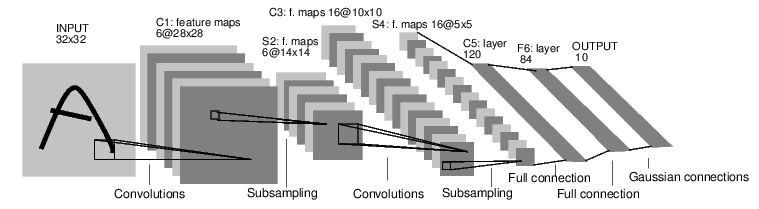
\includegraphics[width=1.0\linewidth]{LeNet.png}
  \end{center}
\end{frame}

\begin{frame}
  \begin{block}{Note!}
    Note -- slight bug in diagram, the image size is 28x28, not 32x32. \\
    The next slide shows the LeNet architecture that we will implement.
  \end{block}
\end{frame}

\begin{frame}
  \frametitle{LeNet Architecture (in more detail)}
  \tikzstyle{c} = [rectangle, draw, fill=blue!20, node distance=1cm, text width=20em, text centered]
  \tikzstyle{p} = [rectangle, draw, fill=purple!20, node distance=1cm, text width=20em, text centered]
  \tikzstyle{f} = [rectangle, draw, fill=green!20, node distance=1cm, text width=20em, text centered]
  \tikzstyle{a} = [rectangle, draw, fill=red!20, node distance=1cm, text width=20em, text centered]

  \begin{center}
    \begin{tikzpicture}[scale=0.5, every node/.style={transform shape}]
      \node [c] (conv2d_1) {Conv2d, 1$\rightarrow$6, 5x5, padding=``VALID''};
      \node [a, below = 0.5cm of conv2d_1] (relu_1) {ReLU};
      \node [p, below = 0.5cm of relu_1] (max_pool_1) {Max Pool, 2x2, stride=2, padding=``VALID''};
      \node [c, below = 0.5cm of max_pool_1] (conv2d_2) {Conv2d, 6$\rightarrow$16, 5x5, padding=``VALID''};
      \node [a, below = 0.5cm of conv2d_2] (relu_2) {ReLU};
      \node [p, below = 0.5cm of relu_2] (max_pool_2) {Max Pool, 2x2, stride=2, padding=``VALID''};
      \node [f, below = 0.5cm of max_pool_2] (fc1) {Fully Connected, 16x4x4$\rightarrow$120};
      \node [a, below = 0.5cm of fc1] (relu_3) {ReLU};
      \node [f, below = 0.5cm of relu_3] (fc2) {Fully Connected, 120$\rightarrow$84};
      \node [a, below = 0.5cm of fc2] (relu_4) {ReLU};
      \node [f, below = 0.5cm of relu_4] (fc3) {Fully Connected, 84$\rightarrow$10};
      \node [a, below = 0.5cm of fc3] (softmax) {SoftMax};
      % Deep Network
      \draw [->] (conv2d_1) -- (relu_1);
      \draw [->] (relu_1) -- (max_pool_1);
      \draw [->] (max_pool_1) -- (conv2d_2);

      \draw [->] (conv2d_2) -- (relu_2);
      \draw [->] (relu_2) -- (max_pool_2);
      \draw [->] (max_pool_2) -- (fc1);

      \draw [->] (fc1) -- (relu_3);
      \draw [->] (relu_3) -- (fc2);
      \draw [->] (fc2) -- (relu_4);
      \draw [->] (relu_4) -- (fc3);

      \draw [->] (fc3) -- (softmax);
    \end{tikzpicture}
  \end{center}
\end{frame}

\begin{frame}
  \frametitle{Activity -- LeNet}
  \Huge{\centerline{\href{https://github.com/sig-ai/tf_workshop/blob/master/demos/mnist.ipynb}{demos/mnist.ipynb}}}
\end{frame}

\section{Extra Resources}
\begin{frame}
  \frametitle{Extra Resources}
  \begin{itemize}
  \item \href{http://cs231n.stanford.edu/}{CS231n -- Recommended for beginners}
  \item \href{https://github.com/Hvass-Labs/TensorFlow-Tutorials}{Extra Tutorial -- If you want more practice using Tensorflow}
  \item \href{http://ufldl.stanford.edu/tutorial/supervised/FeatureExtractionUsingConvolution/}{What is a Convolution?}
  \item \href{http://ufldl.stanford.edu/tutorial/supervised/Pooling/}{What is Pooling?}
  \end{itemize}
\end{frame}

\end{document}